\section{Introduction} 

Designing binding elements for target regions of protein residues or complexes is a hard
computational problem  which has huge impact in biotechnology and pharmaceutical ventures.
This constitutes of drug design and nucleic acid sequence/position weight matrix (PWM)
design. The processes generally employed in solving these kind of problems are traditionally virtual and
experimental screening of large amount of candidate binding elements. These processes are extremely
computationally/experimentally intensive and costly. Moreover, 
most computational methods modeling protein-nucleic acid binding pairs are protein specific models
and lack generalization over protein structures. In this work we propose to provide a generalized
model which can poetntially be used to model protein-nucleic acid binding modeling.
\par
Recently, generative machine learning models have
been used to make significant advances in such tasks. The key generative models that are most
used are mainly of two kind: Variational Autoencoders (VAE) \citep{Kingma2014} and its many
variations \citep{higgins2016beta, sohn2015learning,dilokthanakul2016deep}; Generative Adversarial
Networks \citep{goodfellow2014generative} and variations \citep{wang2018high,zhu2017unpaired}.
For the molecule generation case, \citet{gomez2018automatic} first proposed a variational autoencoder model for drug molecule design.
Similar to RVAgene \red{(cite)} this method encodes training drug molecules represented as SMILES
\citep{weininger1988smiles} string in a regularized latent space which then can be sampled and
decoded to generate new candidate molecules. They also train an additional network to optimize the
generative process based on given chemical properties. This initial model sparked a flurry of folow up 
works mainly addressing various aspects of the problem: e.g. enforcing constraints on the generative process 
such that the generated molecules are chemically valid \citet{kusner2017grammar}, increasing diversity of the generated
molecules, conditional generation etc.  Other models that leverage VAE framework as a drug molecule
generation method consists of \citet{lim2018molecular} (conditional VAE), \citet{dollar2021giving}
(adds attentiona mechanism for more interpretability), \citet{hong2019molecular} (adversarially
regularized VAE) etc. . \citet{kadurin2017drugan} proposed a GAN based generative model
for molecule generation. Other GAN based models
targeting the problem are \citep{de2018molgan} (implicit GAN), \citep{maziarka2020mol} (cycle-GAN), \citet{prykhodko2019novo} (latent vector based GAN), 
\citet{mendez2020novo} (generating hit-like molecules), \citet{guimaraes2017objective} (objective
reinforced GAN) etc. Although most of these methods use the SMILES format representations of a
molecule many deviate from it and propose other forms of representations which helps in increased
validity among the generated molecules. \citet{mitton2021graph} proposes a graph VAE and graph
Transformer \citep{vaswani2017attention} approach for generating molecule graph representations.
\citet{jin2018junction} presents a junction tree base molecule representation and uses the VAE
framework for the geenrative process.
\par
However, when it comes to generative modeling on sequences the amount of research work is sparse and
diverse. VAEs were used recently by \citet{hawkins2021generating} for generating functional protein
variants. \citet{gupta2018feedback} designed a novel feedback GANs for optimizing protein functions.
\citet{berman2020mutagan} presented a seq2seq GAN framework to predict mutations of evolving protein
sequence populations. \citet{linder2020generative} and \citet{killoran2017generating} are deep
generative models geared towards DNA sequence design. An interesting recent work
\citet{yan2021neural} proposes a model for generating RNA sequence and secondary structure. However,
it should be noted that most of these works are very recent and some are still at the pre-print
stage. 
\par
Although, there are works on conditional or property based generation, most of these methods
described above are discovery oriented. However, in this proposal we want to address the problem of
binding element design. Input to our model would be a binding site region on protein surface. And
given that input we want to predict a drug molecule or a sequence position weight matrix (PWM) that
the given binding site could bind to. \hyperref[fig:design_problem]{Fig. 3.1} schematically
describes this problem statement. In the next section, we propose a GAN based method which can
achieve this task.
\begin{center}\begin{figure}
                \makebox[\textwidth]{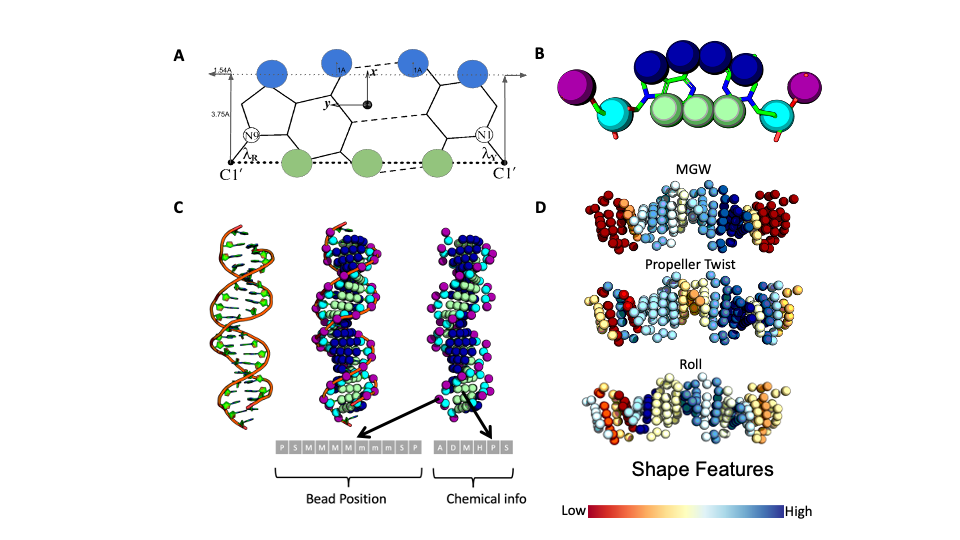
\includegraphics[width=0.8\paperwidth]{design_figs/fig1.png}}
 % archetecture.png: 1149x508 px, 72dpi, 40.53x17.92 cm, bb=0 0 1149 508
        \caption[Binding element design problem schematic]{\textbf{Binding element design problem
        schematic.}}
        \label{fig:design_problem} \end{figure} \end{center}

